\section{Introduction}

Large language model (LLM) agents are increasingly deployed in long-horizon environments where they must maintain state across extended temporal trajectories. Rather than relying solely on transient context windows, modern agent architectures employ persistent memory stores to accumulate experiences, document tool executions, and record intermediate planning states. These stored records actively guide subsequent system behaviors, serving as the knowledge base for downstream retrieval, planning, tool use, and database writes. In this persistent setting, a critical and under-addressed risk is record obsolescence—where a persistent record remains licensed for future reuse after corrective, conflicting, superseding, or policy-relevant evidence has arrived. 

Retrieval alone does not solve this problem. For example, a calendar agent may persistently store that a user has a meeting scheduled on Tuesday. When subsequent email evidence reveals that the meeting has been moved to Friday, the agent must update its memory state. If the agent retrieves the new email and answers the immediate query correctly while leaving the contradicted Tuesday record active in its store, subsequent tasks may retrieve the stale Tuesday record, leading to scheduling conflicts. This silent failure permits immediate query success but leaves a contaminated state that propagates errors in future execution turns.

\begin{figure*}[t]
\centering
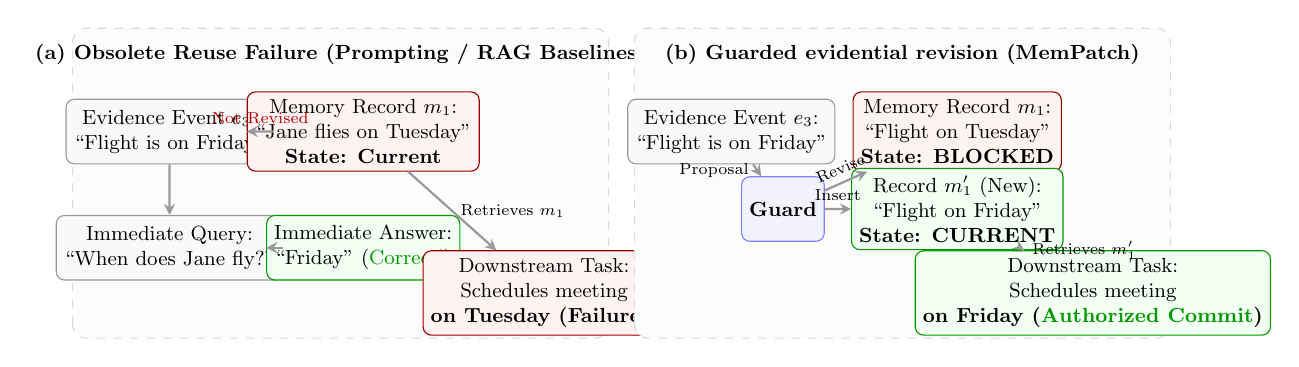
\begin{tikzpicture}[
    scale=0.82, every node/.style={transform shape},
    box/.style={rectangle, draw=gray!80, fill=gray!5, rounded corners=3pt, minimum width=2.4cm, minimum height=1.0cm, align=center, font=\small},
    greenbox/.style={rectangle, draw=green!60!black, fill=green!5, rounded corners=3pt, minimum width=2.4cm, minimum height=1.0cm, align=center, font=\small},
    redbox/.style={rectangle, draw=red!60!black, fill=red!5, rounded corners=3pt, minimum width=2.4cm, minimum height=1.0cm, align=center, font=\small},
    title/.style={font=\bfseries\small},
    arrow/.style={->, >=stealth, thick, draw=gray!80},
    dasharrow/.style={->, >=stealth, dashed, thick, draw=gray!80}
]

% PANEL A: Baseline
\draw[gray!30, fill=gray!2, dashed, rounded corners=5pt] (-0.5,-1.2) rectangle (7.8,3.6);
\node[title] at (3.65,3.2) {(a) Obsolete Reuse Failure (Prompting / RAG Baselines)};

\node[box] (eva) at (1.0,2.0) {Evidence Event $e_3$:\\``Flight is on Friday''};
\node[redbox] (mema) at (4.0,2.0) {Memory Record $m_1$:\\``Jane flies on Tuesday''\\\textbf{State: Current}};
\node[box] (querya) at (1.0,0.2) {Immediate Query:\\``When does Jane fly?''};
\node[greenbox] (ansa) at (4.0,0.2) {Immediate Answer:\\``Friday'' (\textcolor{green!60!black}{Correct!})};
\node[redbox] (downa) at (6.8,-0.5) {Downstream Task:\\Schedules meeting\\\textbf{on Tuesday (Failure!)}};

\draw[arrow] (eva) -- (mema) node[midway,above,font=\scriptsize,text=red!70!black] {Not Revised};
\draw[arrow] (eva) -- (querya);
\draw[arrow] (querya) -- (ansa);
\draw[arrow] (mema) -- (downa) node[midway,right,font=\scriptsize] {Retrieves $m_1$};

% PANEL B: MemPatch
\draw[gray!30, fill=gray!2, dashed, rounded corners=5pt] (8.2,-1.2) rectangle (16.5,3.6);
\node[title] at (12.35,3.2) {(b) Guarded evidential revision (MemPatch)};

\node[box] (evb) at (9.7,2.0) {Evidence Event $e_3$:\\``Flight is on Friday''};
\node[redbox] (membone) at (13.2,2.0) {Memory Record $m_1$:\\``Flight on Tuesday''\\\textbf{State: BLOCKED}};
\node[greenbox] (membtwo) at (13.2,0.8) {Record $m_{1}'$ (New):\\``Flight on Friday''\\\textbf{State: CURRENT}};

\node[box, minimum width=1.0cm, fill=blue!5, draw=blue!50] (guard) at (10.5,0.8) {\textbf{Guard}};

\node[greenbox] (downb) at (15.3,-0.5) {Downstream Task:\\Schedules meeting\\\textbf{on Friday (\textcolor{green!60!black}{Authorized Commit})}};

\draw[arrow] (evb) -- (guard) node[midway,left,font=\scriptsize] {Proposal};
\draw[arrow] (guard) -- (membone) node[midway,above,sloped,font=\scriptsize] {Revise};
\draw[arrow] (guard) -- (membtwo) node[midway,above,font=\scriptsize] {Insert};
\draw[arrow] (membtwo) -- (downb) node[midway,right,font=\scriptsize] {Retrieves $m_1'$};

\end{tikzpicture}
\caption{Comparison of memory integration mechanisms. (a) Traditional agent memory systems retrieve new evidence for immediate queries but leave obsolete records active in memory, causing downstream failures. (b) \method{} routes updates through a deterministic Guard and DPA kernel to revise memory states, preventing stale record reuse.}
\label{fig:motivation}
\end{figure*}

To isolate and evaluate this failure mode, we present \bench{}, a diagnostic benchmark specifically designed to evaluate post-admission validity revision in persistent agent memory. \bench{} requires agents to maintain record-level validity states under chronological evidence streams, scoring updates against hidden ground-truth labels. It evaluates agents not merely on their downstream answers, but on their ability to perform joint revision, scoring the concurrent correctness of task decisions, memory validity states, evidence citations, failure diagnoses, and answers. 

To address this challenge without parameter updates, we propose \method{}, a parameter-free plug-in runtime layer that separates opaque semantic proposals from verifiable persistent-memory transitions. \method{} does not expose the model's latent reasoning. It confines black-box inference to semantic proposal and makes every committed persistent-memory transition explicit, authorization-checked, and replayable. Specifically, \method{} queries a frozen backbone model through a dual-path proposal interface to obtain global states and local typed patches. These proposals are compiled into structured actions and routed through a deterministic, symbolic Revision Guard and a conservative reconciliation function before projecting to memory. 

Empirical evaluations of frozen backbones (Qwen, Gemma, Phi-4, Mistral) show that standard prompting, retrieval-augmented generation (RAG), and memory baselines suffer severe integration failures. By separating semantic proposal generation from deterministic verification, \method{} significantly reduces stale-record reuse and improves memory state consistency without requiring task-specific parameter updates.

This paper makes the following co-equal primary contributions:
\begin{enumerate}[leftmargin=*]
\item \textbf{\bench{}:} A controlled benchmark for evaluating post-admission validity revision. It features record-level validity states, chronological evidence tracking, failure diagnoses, and strict joint evaluation to detect stale memory reuse and integration errors.
\item \textbf{\method{}:} A parameter-free plug-in runtime layer that uses a dual-path proposer interface to separate black-box neural proposals from deterministic, authorization-checked, and replayable memory transitions.
\item \textbf{Empirical Characterization:} An evaluation of frozen models showing that while standard prompting and RAG baselines are vulnerable to stale memory reuse, \method{} consistently enforces safety invariants, reducing the externally unverifiable transition surface to zero.
\end{enumerate}
